% Nicholas R. Jenkins
% Article
% Nicholas R. Jenkins (nicholas.jenkins@email.ucr.edu)
% Department of Political Science
% University of California, Riverside
%
% Manuscript: Minimizing Whose Influence? How Rejecting PAC Contributions Affects Contribution Patterns


% Setup Document and Formatting %
\documentclass[12pt]{article}


\usepackage[utf8]{inputenc}
\usepackage{hyperref}
\usepackage{setspace}
\usepackage[margin=1in]{geometry}
\usepackage[dvipsnames]{xcolor}
\usepackage{bookmark}
\usepackage[english]{babel}
\usepackage{csquotes}
\usepackage{fancyhdr}
\usepackage[bottom]{footmisc}
\usepackage[titletoc,title]{appendix}
\usepackage{tikz}
\usetikzlibrary{positioning}
\usepackage{tabu}
\usepackage{graphicx}
\usepackage{booktabs}
\usepackage{amsfonts}
\usepackage{pdflscape}
\usepackage{footmisc}
\usepackage{caption}
\usepackage{subcaption}
\usepackage{ntheorem}
\usepackage{amsmath}
\usepackage{bm}
\usepackage{longtable}
\usetikzlibrary{shapes, shadows, arrows}
\usepackage{rotating}
\usepackage{multirow}
\usepackage[section]{placeins}
\usepackage{pgfplots}
\usepackage{threeparttablex}
\usepackage{adjustbox}


% Reference Setup %
\hypersetup{
    pdftitle={},    			% title
    pdfauthor={Nicholas R. Jenkins},     		% author
    pdfsubject={},   		% subject of the document
    pdfkeywords={}, 	% list of keywords
    pdfnewwindow=true,      		% links in new window
    colorlinks=false,       			% false: boxed links; true: colored links
    linkcolor=blue,          			% color of internal links
    citecolor=blue,        			% color of links to bibliography
    filecolor=blue,      				% color of file links
    urlcolor=blue           			% color of external links
}


% Bibliography Setup %
\usepackage[authordate, natbib, isbn=false, url=false, doi=false, backend=bibtex]{biblatex-chicago} 
\bibliography{/Users/nickjenkins/Documents/Research/References/BibTeX/biblatex.bib}
    
\DeclareCiteCommand{\citeauthorfirstlast}
  {\boolfalse{citetracker}%
   \boolfalse{pagetracker}%
   \DeclareNameAlias{labelname}{first-last}%
   \usebibmacro{prenote}}
  {\ifciteindex
     {\indexnames{labelname}}
     {}%
   \printnames{labelname}}
  {\multicitedelim}
  {\usebibmacro{postnote}}


% Hypotheses %
\newtheorem{hyp}{Hypothesis}

\makeatletter
\newcounter{subhyp} 
\let\savedc@hyp\c@hyp
\newenvironment{subhyp}
 {%
  \setcounter{subhyp}{0}%
  \stepcounter{hyp}%
  \edef\saved@hyp{\thehyp}% Save the current value of hyp
  \let\c@hyp\c@subhyp     % Now hyp is subhyp
  \renewcommand{\thehyp}{\saved@hyp\alph{hyp}}%
 }
 {}
\newcommand{\normhyp}{%
  \let\c@hyp\savedc@hyp % revert to the old one
  \renewcommand\thehyp{\arabic{hyp}}%
} 
\makeatother


% Title Page Setup %
\title{\textbf{Minimizing Whose Influence? How Rejecting PAC Contributions Affects Contribution Patterns}}

% Solo Author
\author{Nicholas R. Jenkins \\ Department of Political Science\\ University of California, Riverside\\ \href{mailto:nicholas.jenkins@email.ucr.edu}{nicholas.jenkins@email.ucr.edu}}

\date{\today}


% Document %
\begin{document}

% Title Page %
\maketitle
\thispagestyle{empty}

\begin{abstract}
% concisely describe the problem and your solution to it (or the question and your answer to it) and explain why this is a novel contribution. Carefully draft each sentence in the abstract to efficiently convey all the important information about your paper

Do pledges to reject corporate PAC contributions minimize corporate influence in elections? I address this question with campaign finance data for Congressional candidates in the 2018 elections. While I find that candidates who pledge to reject corporate PAC contributions receive fewer contributions from business PACs, I also find that they substitute these funds with small-dollar contributions, large-dollar contributions from individuals affiliated with business interests, and large-dollar contributions from individuals outside their districts. These findings support the claim that voters are motivated to donate by anti-corporate PAC pledges, as candidates hope, but that these candidates likely substitute corporate PAC contributions with funds from sources beyond small-dollar donations. This study is the first to examine the effects of rejecting corporate PAC contributions on contribution patterns and the first test of the claim that anti-corporate PAC pledges will increase small-dollar donations.

\medskip

\noindent \textbf{Key Words:} Campaign Finance; Elections; Political Action Committees; Small Donors

\end{abstract}

\pagebreak

\cleardoublepage
\setcounter{page}{1}

\doublespacing

% Section 1: Introduction  %
\section{Introduction} \label{sec: intro}

During the Democratic debate on February 6, 2016, Bernie Sanders stood on stage and enthusiastically announced to the audience, ``I am very proud to be the only candidate up here who does not have a super PAC, who’s not raising huge sums of money from Wall Street and special interests." Sanders publicly voiced his opposition to corporate Political Action Committee (PAC) contributions and refused their support in contrast to his Democratic opponent, Hillary Clinton, who accepted over \$1.7 million from PACs; a decision for which she faced sharp criticism from voters on the left \citep{seitz-wald2015}. 

The strategy of rejecting corporate PAC contributions continued into the 2018 and the 2020 elections as well. OpenSecrets News reported that 52 members of the 116th Congress, including 35 non-incumbents, announced that they would not accept money from corporate PACs during their campaigns \citep{evers-hillstrom2018}. Similarly, an article in ABC News claimed, ``The 2020 Democratic presidential candidates are forgoing corporate money in an effort to capture small donors'' \citep{harper2019}. All 14 of the 2020 presidential Democratic candidates declined to accept corporate PAC contributions although only three declined to accept all PAC contributions. 

Candidates who seek small-dollar donations in place of PAC contributions are responding to a demand from voters wanting to bring the era of ``captured" politicians to an end \citep{culberson2019}. Many voters believe that corporate PAC contributions are corrupt and lessen the desire of elected officials to serve their constituents. ``We desperately need to get the money out of the political system. Because I don’t think we have a Congress that’s representing the people anymore," a Minnesota resident complained during the 2018 midterm \citep{stockman2018}. When asked about rejecting corporate PAC money, Beto O’Rourke's communications director said, ``It’s a major theme of the campaign. People want to know that you are going to respond to them and their interests, and not the most recent check you received" \citep{stockman2018}. However, elections are expensive, and refusing corporate PAC contributions suggests that candidates anticipate the ability to substitute corporate money with funds from other sources.

Despite the intentions of anti-corporate PAC pledges, do they limit corporations' influence in elections? I argue that while these pledges motivate small-dollar contributions, corporations may pursue alternative contribution strategies for these candidates rather than cease their contribution activity altogether. I show that candidates who reject corporate PAC contributions tend to receive more individual contributions of less than \$200, indicating that these pledges help candidates' get-out-the-small-dollar-donations efforts. Additionally, I show that candidates who make anti-corporate PAC pledges tend to receive fewer business PAC contributions, but they are tend to receive more contributions from individuals affiliated with business interests. Finally, I show that candidates who make the anti-corporate PAC pledge receive more contributions from individuals affiliated with business interests outside their district suggesting that candidates who pledge to reject corporate PAC contributions substitute contributions from other sources. These findings indicate that although anti-corporate PAC pledges may reduce PAC activity, they do not prevent corporations from pursuing alternative ways to exert their influence in elections. 

This study makes two significant contributions. First, this is the only study so far to examine the effects of pledging to reject corporate PAC contributions. To continue advancing our understanding of how outside actors use money to influence politics, we must investigate evolving strategies of making and soliciting contributions. This study provides a foundation for future research to build on.   

Second, this study is the first to test the claim that candidates increase the number of small-dollar donations from individual voters by pledging to reject corporate PAC contributions. Given the cost of running for office, the decision to reject corporate PAC contributions suggest that candidates believe that they will attract more small-dollar donations from individuals by publicizing their opposition to PACs. 

Refusing corporate PAC contributions may result in less transparency about candidates' funding sources since corporate interests are unlikely to simply stop their involvement in politics. Bundled contributions made through corporate individuals require more extensive research to identify, and mounting pressure from voters to reject these contributions may increase outside spending and push corporations into the arena of ``dark money" \citep{opensecrets.org2019, massoglia2021}. If this happens, it will be far more difficult to monitor corporate electioneering.


\section{Voter Perceptions and Corporate Influence}

Whether a candidate refuses corporate PAC contributions as a matter of principle or electoral strategy is challenging to know. It is, however, very plausible that strategic benefits outweigh any idealistic concerns. Candidates presumably adopt the anti-corporate PAC strategy with the belief that it will not result in electoral defeat, and it is undoubtedly the case that Americans are skeptical about money in politics \citep{lubenow2001}. Previous research finds that when questioned, voters typically perceive corporations' contributions as more corrupt than those made by individuals and consider small-dollar contributions as the most honest \citep{bowler2016}. Thus, the sources of campaign funding matter to some voters, and attempts to distance oneself from ``corrupt" sources may prove electorally advantageous. 

In effect, making an anti-corporate PAC pledge may serve as a signal of ``trustworthiness." Indeed, these types of signaling effects have been well-documented elsewhere in the political science literature (e.g., \citet{iyengar1989}). Ella \citet{nilsen2019} reported that Elizabeth Warren ``swore off PAC money to make a statement" in a story for Vox.com. In an email to her supporters, Warren explained, ``For every time you see a presidential candidate talking with voters at a town hall, rally, or local diner, those same candidates are spending three or four or five times as long with wealthy donors — on the phone, or in conference rooms at hedge fund offices, or at fancy receptions and intimate dinners — all behind closed doors" \citep{nilsen2019}. In 2020, Democratic candidates were almost in competition to distance themselves as far as they could from PACs and special interests, and there is little reason to suspect that the 2018 Democratic candidates viewed this issue any differently. 

Rejecting corporate PAC contributions may motivate individual small donors, but whether it also meets the goal of reducing corporate influence is unclear. Campaign costs are enormous and continually rising, meaning that candidates who forgo contributions from corporate PACs will need to substitute these lost funds with those from other sources. Moreover, given the opportunity costs corporations face from not getting involved in elections \citep{denzau1986, kroszner1998}, it would be economically irrational for a corporate PAC to abandon its efforts because a candidate wishes to avoid the negative publicity of receiving contributions from their affiliated PACs. Instead, a rational PAC will use alternative means to make campaign contributions. 

One such alternative is to fund candidates directly with large-dollar donations and corporately-bundled individual donations. In fact, the Center for Responsive Politics (CRP) documents donations made by individuals in connection with larger organizations because, ``In some cases, a cluster of contributions from the same organization may indicate a concerted effort by that organization to `bundle' contributions to the candidate" \citep{opensecrets.org}. To put this into context, contributions to all candidates from business PACs totaled \$394 million in the 2018 election cycle compared to over \$1.6 billion from individuals affiliated with business interests \citep{opensecrets.org2021}. This type of giving strategy would allow recipients to claim that they do not accept corporate PAC money while still receiving corporate support. 

Candidates who adopt this strategy likely do so either because they feel confident that they can win without corporate PAC support or adequately compensate for the loss of funds with those from other sources. ``Other sources" could be small-dollar donations, party organizations, or super PACs. Small-dollar donations, however, are unlikely to be substantial enough for most candidates to be competitive. Moreover, given the incentives for corporations to participate in politics, they will likely find alternative means to finance their preferred candidates.


\section{Data, Methods, and Results}

To evaluate anti-corporate PAC pledges, I take advantage of unique campaign finance data on Congressional candidates in the 2018 midterm election provided by The Center for Responsive Politics at \href{https://www.opensecrets.org}{Opensecrets.org.} These data are unique because The Center for Responsive Politics (CRP) is the first organization, to my knowledge, to keep records on which candidates pledged not to accept corporate PAC contributions for the 2018 elections. Unfortunately, this limits my sample to only the 2018 midterm as earlier data is not available.\footnote{Data for the 2020 election cycle is not currently available.} Additionally, the CRP only records pledges for candidates who won their elections.

The final sample has data for 259 members from 45 different states of which 33 percent are freshmen and almost 22 percent pledged to refuse corporate PAC contributions. Of the candidates who made the anti-corporate PAC pledge 35 were freshmen and and 13 were returning members. Figure \ref{fig: nominate plot} shows the DW-Nominate scores for Democrats in the sample by whether or not they reject corporate PAC money. Members who take the pledge are fairly representative of their party as a whole and are, surprisingly, slightly more moderate than their corporate PAC-accepting peers on the first dimension scores. 

\begin{figure}[!htb]
    \centering
    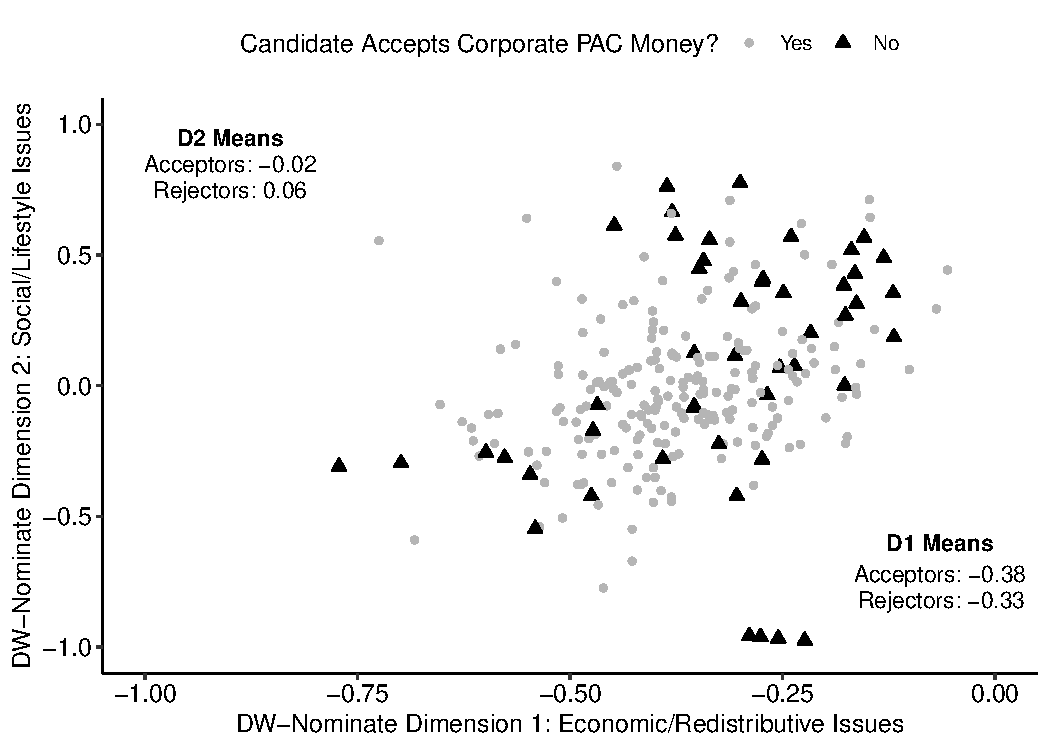
\includegraphics[width=0.75\linewidth]{nominate_plot.pdf}
    \caption{DW-Nominate Scores of Democrats in the Sample by Position Towards Corporate PAC Money.}
    \label{fig: nominate plot}
\end{figure}

To investigate the substitution of contributions from one source to another, I focus on contributions from business PACs, small-dollar individual contributions, and large-dollar individual contributions. Campaign contributions are typically categorized into three main groups; business, labor, and ideological PACs. Business PAC contributions are defined as contributions made from industries other than education, ideological/single-issue organizations, labor organizations, or political organizations, as categorized by the CRP. Business PAC contributions are the corporate PAC contributions that anti-corporate PAC pledges aim to reject.   

Small-dollar individual contributions are classified by the CRP as contributions of less than \$200 since the Federal Election Commission only requires itemized receipts of contributions made from individuals that exceed \$200. Large-dollar individual contributions are typically defined as contributions made by individuals of \$200 or more, and the CRP classifies each contribution by industry according to the donor's employer. The CRP is unique in classifying campaign contributions by industry. They argue that individual contributions could be used to represent corporate interests, and the fact that the FEC requires the disclosure of a donor's employer for contributions over \$200 indicates a fear of influence \citep{opensecrets.orga}. The CRP has also found that donors who give more than \$200 are regularly corporate executives and not lower-level employees. 

To narrow in on a measure of corporate influence through individual donations, and because the CRP has observed that individuals who give more than \$200 are often corporate executives, I calculate the total contributions from individuals who work in business industries and give \$1,000 or more.\footnote{See \href{https://www.opensecrets.org/resources/faq/}{https://www.opensecrets.org/resources/faq/} for details on how and why the CRP tracks the industry of individual contributors.} Thus, my measure of large-dollar individual contributions, which I will refer to as individual business contributions, is contributions of \$1,000 or more made by individuals who are employed in a business industry which includes all contributions from OpenSecrets industry codes except those for ideological, partisan, and labor organizations. Finally, to gauge business influence from outside a member's district, I calculate the total number of individual business contributions made from outside of the district for which a candidate is running.  

Before reviewing the results, it is crucial to clarify the goal of these analyses. My study design does not meet the criteria to make credible causal inferences, but this does not undermine its value. There are two plausible causal mechanisms that my research design is unable to differentiate between. First, making an anti-corporate PAC pledge may cause a candidate to receive more contributions from business individuals. Alternatively, candidates may make the pledge because they know they can raise the money that the need from other sources. Regardless of which is true, both mechanisms indicate that the anti-corporate PAC is not a virtuous as the candidates making them would like us to believe. 

Independent of causality, this study aims to establish a set of descriptive findings to lay a foundation for future work. Anti-corporate PAC pledges have yet to receive scholarly attention, even though more candidates than ever make them and they are widely publicized. Given how little we know about the consequences of these pledges, this study marks the first exploration into an increasingly salient campaign strategy. Moreover, my findings are suggestive of the possibility that corporations continue to exert their influence through individual donations.

\begin{figure}[!ht]
    \centering
    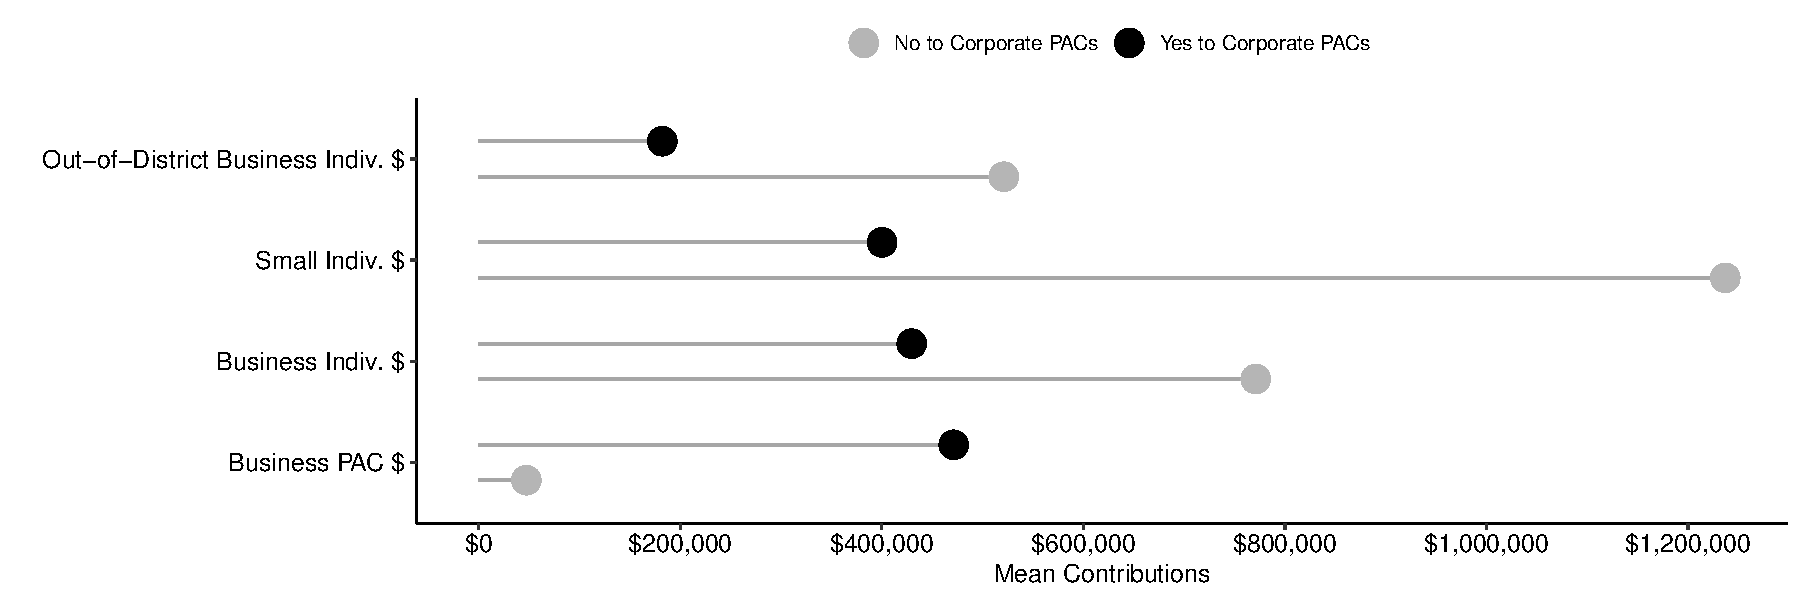
\includegraphics[width=0.9\linewidth]{all_candy.pdf}
    \caption{Contributions to Candidates by Source and Whether or not they Reject PAC Contributions.}
    \label{fig: all contribs}
\end{figure}

Figure \ref{fig: all contribs} displays the mean contributions across candidates by whether or not they pledge to reject corporate PAC contributions. It shows that candidates who take the pledge receive almost zero contributions from business PACs, as expected. However, these candidates receive more individual business contributions (contributions from individuals that work in a business industry of \$1,000 or more) and out-of-district business individuals.  Finally, while candidates who take the pledge also receive higher small-dollar individual contributions (individual contributions of less than \$200), this type of giving only accounts for 23 percent of their total campaign receipts (small-dollar individual contributions account for 14 precent of total campaign receipts for candidate who do not make the pledge). Looking at contributions from all sources in Figure \ref{fig: total money}, candidates who refuse corporate PAC contributions receive and spend a lot more money, on average, than their corporate PAC-accepting colleagues. 

\begin{figure}[!ht]
    \centering
    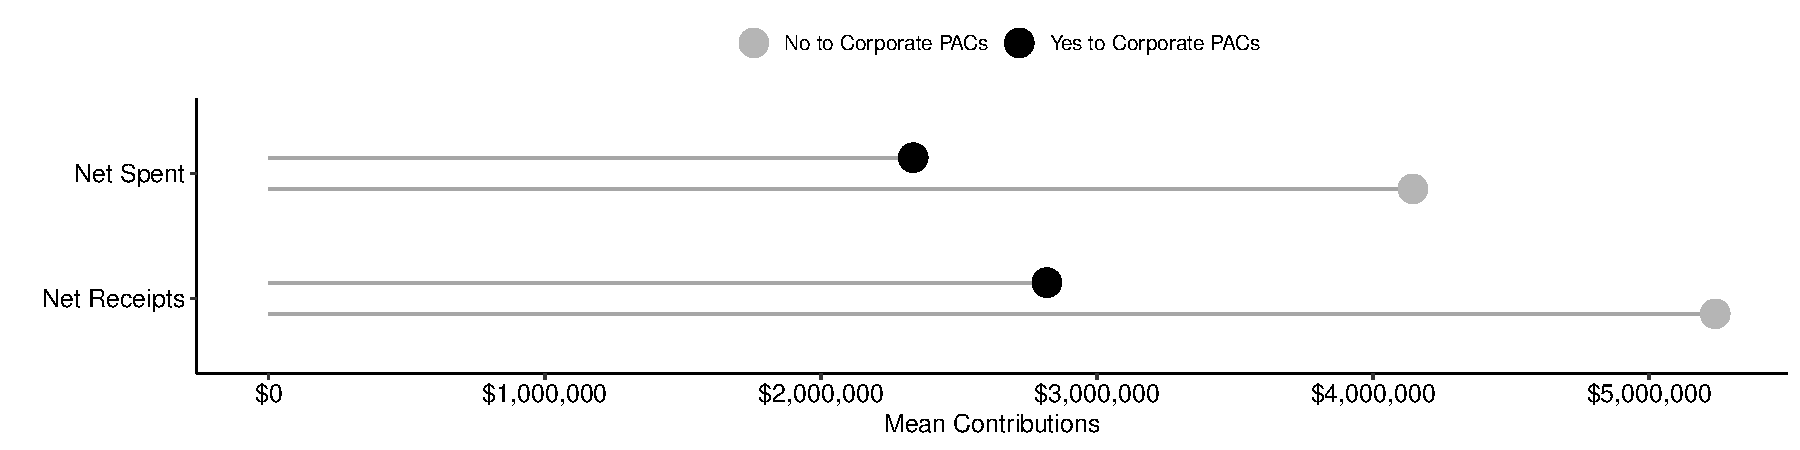
\includegraphics[width=0.9\linewidth]{spending_candy.pdf}
    \caption{Contributions to Candidates by Source and Whether or not they Reject PAC Contributions.}
    \label{fig: total money}
\end{figure}

To examine the substitution effect of campaign contributions, my primary interest is in how the composition of a member's campaign contribution sources change in response to making an anti-corporate PAC pledge. To model this process, I use a Dirichlet likelihood function. Because the Dirichlet distribution is a multivariate generalization of the beta distribution, it allows me to simultaneously model the proportion of total contributions each member receives from business PACs, business individual, small-dollar, and out-of-district business individual contributions as a function of a set of predictors. By estimating these proportional changes, this model allows me to describe how members substitute business PAC contributions with those from other sources. This model is defined as follows: 
$$
\begin{aligned}
\bm{Y} &\sim \text{Dirichlet}(\bm{\mu_i}, \phi) \\
\eta_{c,i} &= \bm{x_i}^\top \bm{\beta_c} \\
\mu_{c,i} &= \frac{\exp(\eta_{c,i})}{\sum^{C}_{d=1}\exp(\eta_{i,d})} \\
\end{aligned}
$$

\noindent where $c$ indexes the components, $d$ is the dimension of the simplex, $\bm{Y}$ is a matrix composed of the proportion of contributions received by each candidate from business PACs, business individual, small-dollar, and out-of-district business donations, and $\bm{x_i}$ is a matrix of predictors for each outcome variable for each candidate. The linear combination of $\eta_{c,i}$ is mapped to $\mu_{c,i}$ with the multivariate logit link function.\footnote{For more details on the derivation of the Dirichlet model, see \citet{hijazi2009}.} This model was estimated in Stan using Hamiltonian Monte Carlo with weakly informative priors, 4 chains, run for 4,000 iterations, and a warmup period of 2,000 iterations. The model's convergence is indicated by a visual inspection of the trace-plots and each parameter's $\hat{R}$ value being less than 1.01 \citep{standevelopmentteam2021, burkner2017a}. 

One limitation of the Dirichlet likelihood, is that it is only defined for positive real number outcomes $y \in  \mathbb{R}^+$ and some candidates in the sample received zero contributions from one or more sources. To overcome this problem, I adopt two different strategies. First, I drop all zero values from the data set and estimate the Dirichlet model on positive non-zero outcomes. Second, I use a zero-augmented gamma likelihood to model contributions from each source individually. The results from the zero-augmented models are provided in Appendix \ref{sec: zip model}. Both models yield consistent evidence in support of my argument that candidates who refuse corporate PAC contributions substitute them with contributions from other sources. 

I model the composition of each candidate's contributions as a function of whether or not they pledge to reject corporate PAC contributions (candidates who accept corporate PAC contributions are the reference group) and several adjustment variables, which include a 0-1 indicator for a new member, the percentage of the district that is white, the percentage of the district that is black, the percentage of the district that is Latino, the percentage of the district that is Asian, the percentage of the district's population with a bachelors degree, Hilary Clinton's share of the district vote in 2016, the share of the district vote for Democratic House candidates in 2016, the voting-age population in the district, and the median household income of a district. To aid with interpretation, I center all continuous variables by subtracting the mean and dividing by two standard deviations \citep{gelman2020}.

\begin{figure}[!htb]
    \centering
    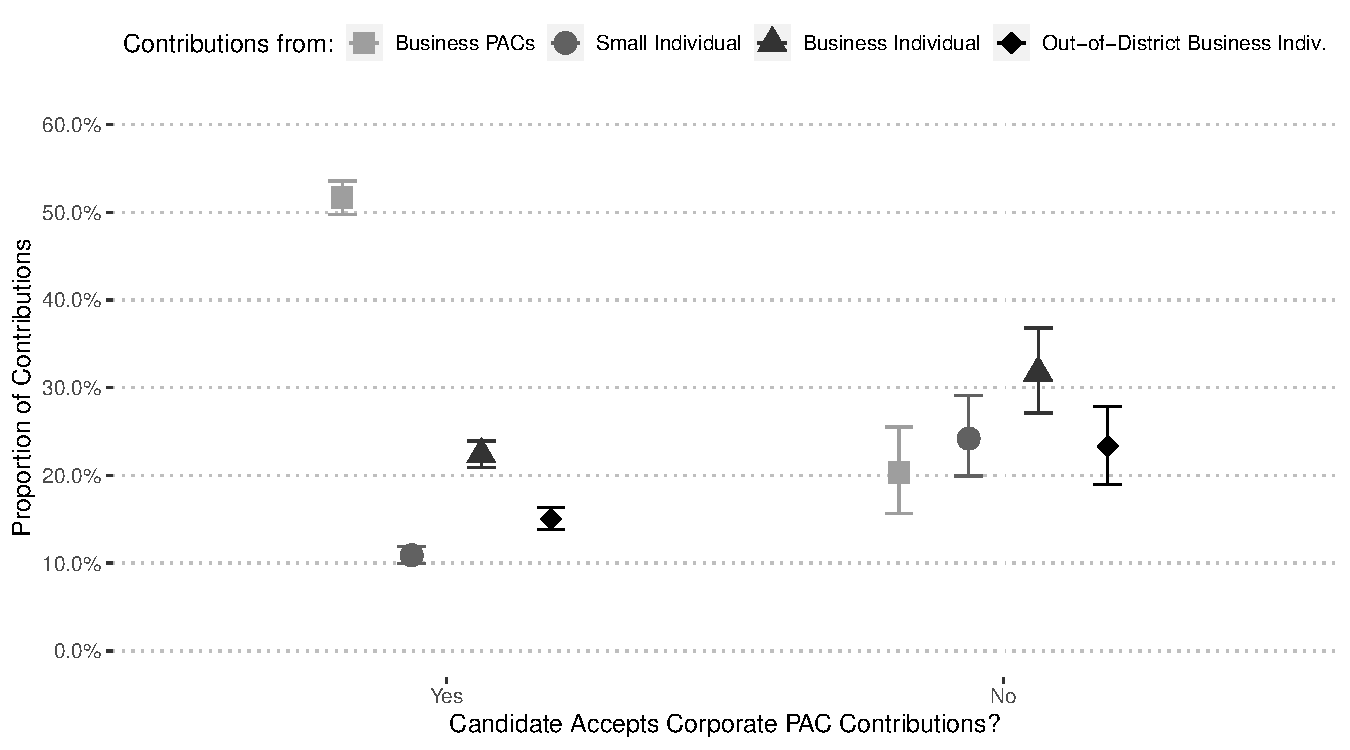
\includegraphics[width=0.9\linewidth]{dir_model_results.pdf}
    \caption{\textbf{Estimate Composition of Campaign Contributions by Corporate PAC Position.} This figure displays the median point estimates of the Dirichlet model with 90\% credible intervals. Analyses use four Markov chain Monte Carlo (MCMC) chains at 4,000 iterations each with a warmup period of 1,000 samples using the Hamiltonian Monte Carlo algorithm. All chains indicate convergence with every $\hat{R}$ value being less than 1.01.}
    \label{fig: dir results}
\end{figure}

Figure \ref{fig: dir results} displays the results of the Dirichlet model.\footnote{Figure \ref{fig: dir results} displays 90\% intervals rather than 95\% because of the relatively low effective sample sizes for each coefficient. \citet{kruschke2014} suggests only using 95\% credible intervals when the effective sample size is at least 10,000 to ensure a reasonably accurate estimate of the highest density region.} It summarizes the estimated proportion of contributions from each source that a candidate is predicted to receive conditioned on whether or not they pledge not to accept corporate PAC contributions and the adjusting variables. Candidates who accept corporate PAC contributions are estimated to receive over 50 percent of contributions from business PACs (estimate = $1.55$, Pr(+) $>$ 99.9\%, 90\% HDI [$1.44, 1.66$]) compared to around 20 percent for candidates who refuse them (estimate = $-1.73$, Pr(+) $>$ 99.9\%, 90\% HDI [$-2.07, -1.39$]). In addition to this expected decrease in business PAC contributions, candidates who pledge to reject corporate PAC contributions receive a higher proportion of contributions from small-dollar (estimate = $1.73$, Pr(+) $>$ 99.9\%, 90\% HDI [$1.36, 2.07$]), business (estimate = $1.28$, Pr(+) $>$ 99.9\%, 90\% HDI [$0.94, 1.61$]), and out-of-district business individual contributions (estimate = $1.37$, Pr(+) $>$ 99.9\%, 90\% HDI [$1.04, 1.73$]). The largest proportional shift is for contributions from small-dollar individuals. Candidates who accept corporate PAC contributions are predicted to receive just over 10 percent of their contributions from small-dollar donors compared to around 25 percent for candidates who refuse corporate PAC money. Similarly, candidates who refuse corporate PAC contributions are predicted to receive around 30 and 25 percent of their contributions from business (contributions from individuals that work in a business industry of \$1,000 or more) and out-of-district business individual contributions. 

These results suggest that anti-corporate PAC pledges are associated with increased support from small-dollar donors. This finding bolsters the claim that anti-corporate PAC pledges motivate voters to make small donations and is as Democrats seemed to have expected. However, the results are also consistent with the claim that anti-corporate PAC pledges do not reduce corporate influence in elections. Instead, these pledges are associated with alternative corporate contribution strategies. More individuals who work in business industries make non-trivial contributions ($\geq$ \$1,000) to candidates who pledge to reject corporate PAC contributions, and these candidates are supported by more contributions from outside of their district. Rather than abandoning their efforts to influence politics, corporations seem to continue supporting candidates who refuse corporate PAC money by making bundled contributions through individuals who live within, and outside of, a candidate's district.


\section{Conclusion} \label{sec: conclusion}

The strategy of rejecting corporate PAC contributions is puzzling and has yet to receive academic investigation. Although candidates advertise this strategy as an attempt to finance their campaigns with small-dollar donations and thwart corporate influence, it is unclear whether it is successful in accomplishing either of these goals. Furthermore, it is unlikely that candidates would refuse corporate PAC contributions without any strategic considerations since they would not do so if they thought it would result in an electoral defeat. 

This paper offers evidence that refusing corporate PAC contributions galvanizes small-dollar donations but may not reduce corporate influence. Instead, anti-corporate PAC pledges are associated with alternative corporate contribution strategies. Specifically, candidates who reject corporate PAC contributions are predicted to receive fewer contributions from business PACs, but they are also predicted to receive more contributions from individuals who contribute \$1,000 or more and work in a business industry. Moreover, Candidates who refuse corporate PAC contributions are also predicted to receive more individual contributions of \$1,000 or more from outside their district.   

Future work will be needed to determine whether these findings generalize to other elections, and causal research designs can uncover the mechanisms at play. Still, my findings are suggestive of the claim that corporations pursue strategies of influence through individual contributions when candidates refuse to accept their PAC's contributions. 

Ironically, refusing corporate PAC contributions may create a campaign finance system that is less transparent and more difficult to understand. Political action committees are regulated entities, often with clear sponsors, that require disclosures of donors and contribution recipients. While it takes some effort, voters can generally identify a candidate's PAC contributors and have some idea of what the group stands for. If public opinion on PAC contributions sours, the organizations these PACs represent may resort to less transparent strategies like the use of super PACs, 527 committees, and ``dark money;" indeed emerging evidence suggests that this is already happening \citep{opensecrets.org2019, massoglia2021}. Also, if anti-corporate PAC strategies entail a higher reliance on large-dollar contributions from individuals outside a candidate's district, it becomes less obvious whom these members are actually representing (e.g., \citet{baker2016}). If we are to develop a more robust understanding of how money is used to influence the political process, we must continue investigating the evolving ways individuals and groups make, and how members solicit, campaign contributions. 

\singlespacing
\pdfbookmark[1]{References}{References}
%\bibliography{/Users/nick/Documents/Research/Articles/reference.bib}
\printbibliography
\pagebreak


\begin{appendices}
\doublespacing
% Set Tables Names to have "A" Before the Table Names
\setcounter{table}{0}
\renewcommand{\thetable}{A\arabic{table}}

\section{Zero-augmented Gamma Estimation} \label{sec: zip model}

As an alternative to using the Dirichlet likelihood to model the composition of a member's campaign contributions, I model the data generating process of each type of campaign contributions with a gamma likelihood function since the gamma distribution describes a data generating process for a random variable with only positive real number outcomes $y \in  \mathbb{R}^+$. However, because some candidates pledge to reject PAC contributions, contribution values of zero are also possible. A zero could result either because they accept zero contributions from a group or because a group decides not to contribute to a candidate. 

\begin{figure}[!htb]
    \centering
    \footnotesize
    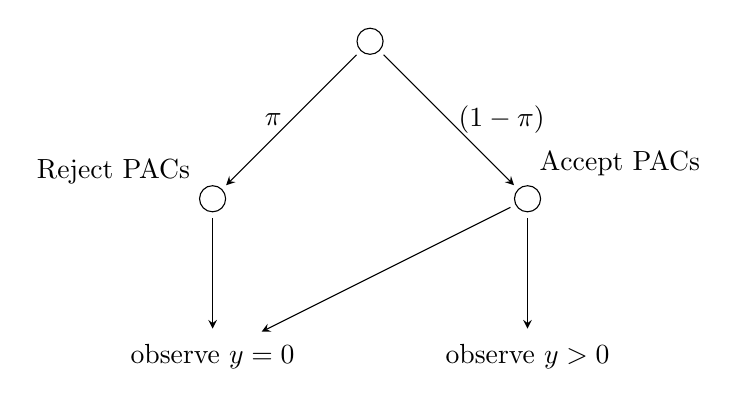
\begin{tikzpicture}[
        node distance=2.0cm,
      scale=0.5,
      level/.style={thick},
      virtual/.style={thick,densely dashed},
      trans/.style={->,shorten >=2pt,shorten <=2pt,>=stealth},
      classical/.style={thin,double,<->,shorten >=4pt,shorten <=4pt,>=stealth}
    ]
    \node(a)[circle, draw=black, label={160:Reject PACs}] {};
    \node(z)[right of=a] {};
    \node(b)[circle, draw=black, right of=z, label={80:Accept PACs}] {};
    \node(c)[circle, draw=black, above of=z] {};
    \node(d)[below of=a] {observe $y = 0$};
    \node(e)[below of=b] {observe $y > 0$};
    
    \draw [trans] (c) -- (a) node[midway, left] {$\pi$};
    \draw [trans] (c) -- (b) node[midway, right] {$(1 - \pi)$};
    \draw [trans] (a) -- (d);
    \draw [trans] (b) -- (e);
    \draw [trans] (b) -- (d);
    \end{tikzpicture}
    \caption{Zero Generation Process.}
    \label{fig: zero process}
\end{figure}

This dual process is summarized in Figure \ref{fig: zero process}. Candidates decide to reject PACs with a probability of $\pi$ or accept PACs with probability $(1 - \pi$). If they reject PACs, we observe a zero. If they accept PAC contributions, we may still observe a zero if the candidate receives zero donations from the group in question. However, because the gamma distribution is not defined for zero values, I use a zero-augmented gamma likelihood for models of contributions that contain zero values. In the data, 9 percent of candidates received zero contributions from out-of-district business individuals and 4 percent received zero contributions from business PACs.

The zero-augmented gamma likelihood is a mixture of bernoulli and gamma distributions and is easily summarized as $\text{ZGamma}(\pi, \mu, \theta)$ where $\pi$ indicates the probability of a zero, and non-zero outcomes are described by a mean $\mu$ and rate $\theta$.\footnote{For more information on the mathematical details, see \citet{mccullagn1989}} An alternative solution to model this data would be to model cases of zero contributions separately from non-zero cases, but this approach would sacrifice information about the relationship between these cases. By leaving zero cases in the dataset, the model can more accurately capture the data generating process. Formally the model is defined as:
$$
\begin{aligned}
    y_i &\sim \text{ZGamma}(\pi_i, \mu_i, \theta_i) \\
    \log \left( \frac{\pi_i}{1 - \pi_i} \right) &= \alpha_{\pi} + \beta_{1\pi} (\text{No PACs})_i + \beta_{2\pi} (\text{New Member})_i \\
    \log(\mu_i) &= \alpha_{\mu} + \beta_{1\mu} (\text{No PACs})_i + \bm{X} \bm{\beta_{\mu}} \\
\end{aligned}
$$

\noindent where $i$ indexes individuals, $\bm{X}$ is a matrix of adjustment variables, and $\bm{\beta_{\mu}}$ is the corresponding coefficient vector. The probability of receiving contributions is modeled as a function of both rejecting PACs and being a new member  \citep{brunell2005, biersack1993}.\footnote{To model campaign contributions for outcomes without zeros (small-dollar individual, large-dollar individual, business individual, total individual), I use a standard gamma likelihood. All models are estimated with weakly-informative priors to better approximate large-n estimates \citep{mcneish2016} and because using ``uninformative" priors is seldom justified since one always knows something \textit{a priori} about the range of plausible values \citep{gelman2008a}.} These models were estimated in Stan using Hamiltonian Monte Carlo with weakly informative priors, 4 chains, run for 4,000 iterations, and a warmup period of 2,000 iterations. The model's convergence is indicated by a visual inspection of the trace-plots and each parameter's $\hat{R}$ value being less than 1.01. 

\begin{figure}[!htb]
	\centering
	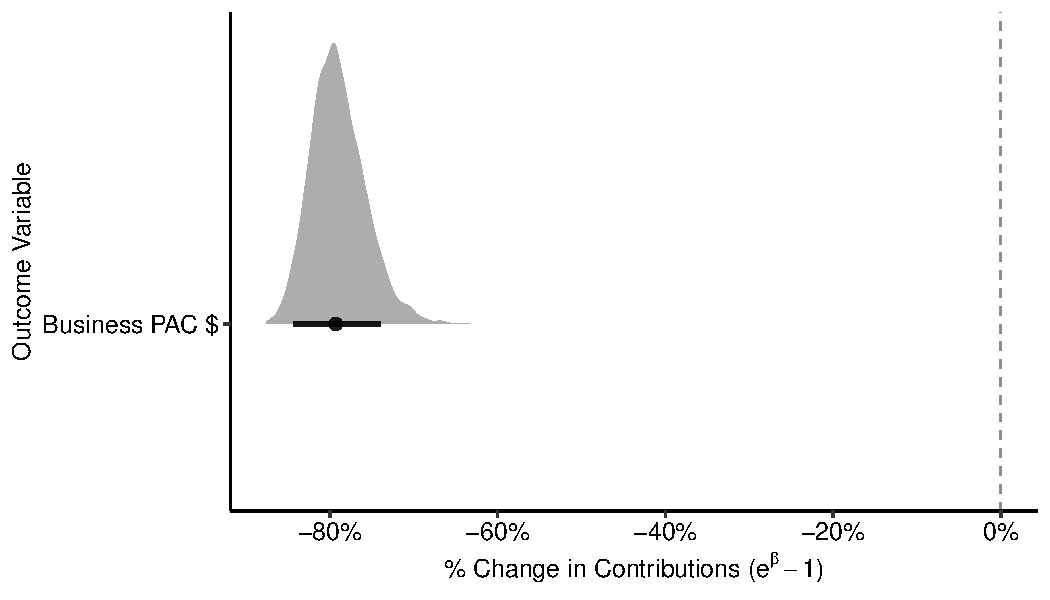
\includegraphics[width=0.9\linewidth]{pac_gamma_coef.pdf}  
  	\caption{Model Estimates for Rejecting Corporate PAC Contributions and Contributions from Business PACs}
	\label{fig: pac results}
\end{figure}

Figure \ref{fig: pac results} visualizes the results of the first model estimating total business PAC contributions received as a function of whether or not a candidate pledges to reject corporate PAC contributions and adjustment variables. Compared to candidates who do not pledge to reject corporate PAC contributions, candidates who take the pledge are expected to have about an 80 percent decrease in business PAC contributions.\footnote{$(e^{-1.57}) - 1 \approx -0.792$.} The probability that this coefficient is positive is greater than 99.9 percent (estimate $= -1.57$, 90\% HDI [$-1.82, -1.32$]).\footnote{I use 90\% intervals rather than 95\% because of the relatively low effective sample sizes for each coefficient. \citet{kruschke2014} suggests only using 95\% credible intervals when the effective sample size is at least 10,000 to ensure a reasonably accurate estimate of the highest density region.} This evidence supports the claim that candidates stay true to anti-corporate PAC pledges. 

Do candidates, however, substitute corporate PAC contributions with contributions from other sources? The next set of results examines contributions from other sources. Figure \ref{fig: indiv results} visualizes the results of models estimating the total amount of small-dollar individual donations ($<$ \$200), individual business contributions ($\geq$ \$1,000 from an individual employed in a business industry), and out-of-district individual business contributions. Candidates who reject corporate PAC contributions are predicted to have a significant increase in small-dollar donations (estimate = 1.03, Pr(+) $>$ 99.9\%, 90\% HDI [$0.70, 1.34$]). Specifically, the model predicts an increase of about 180 percent. 

\begin{figure}[!htb]
	\centering
	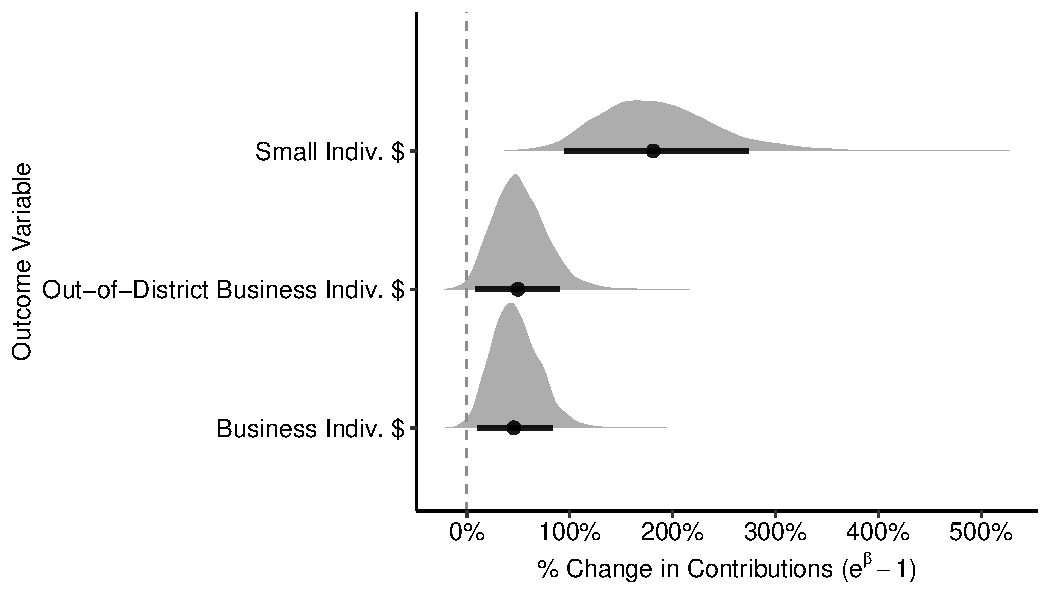
\includegraphics[width=0.9\linewidth]{indv_gamma_coef.pdf}  
	\caption{Model Estimates for Rejecting Corporate PAC Contributions and Contributions from Business PACs}
	\label{fig: indiv results}
\end{figure}

In addition to the expected increase in small-dollar individual donations, candidates who take the pledge are also predicted to have more contributions from business individuals in total and from outside for their districts. Individual business contributions are expected to increase almost 46 percent (estimate $= 0.37$, Pr(+) $>$ 99\%, 90\% HDI [$0.12, 0.61$]). Similarly, out-of-district individual business contributions are predicted to increase by 49 percent (estimate $= 0.40$, Pr(+) $>$ 98\%, 90\% HDI [$0.14,  0.70]$).  

In sum, the results from these models are consistent with those of the Dirichlet model.

\end{appendices}


\end{document}
